\documentclass{article}
\usepackage[utf8]{inputenc}
\usepackage{tikz}
\usepackage{pgfplots}
\usetikzlibrary{arrows}
\usetikzlibrary{shapes.arrows}
\usetikzlibrary{fit}
\title{Some tikz examples}
\author{Francesca Diedolo }
\date{September 2022}

\begin{document}

\maketitle

\section{Introduction}
Tikz is a very power tool to create grphical content in Latex. 
Here are some examples for an easier get started.

Some simple channel models:
\begin{figure}[ht]
\centering
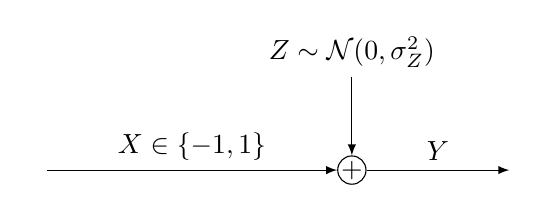
\begin{tikzpicture}
    \node(src){};
    \node[circle, draw, inner sep=0cm]at (4,0) (plus){$+$};
	
	\node at (4,1.5)(z){$Z\sim\mathcal{N}(0,\sigma_Z^2)$};

	\draw[-latex] (src) --  (plus) node[midway,above] {$X\in \{-1, 1 \}$};
	\draw[-latex] (plus) -- node[midway,above] {$Y$} (6,0);	
	
	\draw[-latex](z)--(plus);
\end{tikzpicture}
\end{figure}


\begin{figure}[h]
    \centering
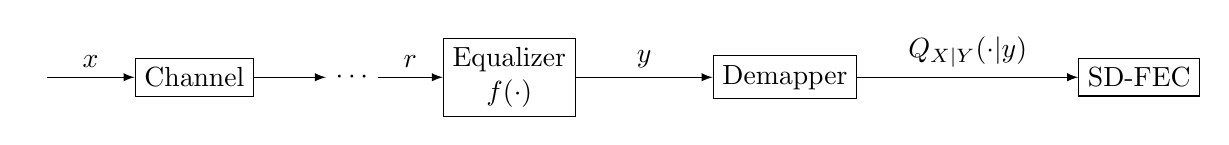
\begin{tikzpicture}
		\node(src) at (0,0){};
		\node[draw] at (2,0) (ch) {Channel};
		\node at (4,0) (dsp) {$\cdots$};
		\node[draw, align=center] at (6,0) (nleq) {Equalizer \\ $f(\cdot)$};
		\node[draw] at (9.5,0) (demap) {Demapper};
		\node[draw] at (14,0) (fec) {SD-FEC};
		
		\draw[-latex] (src) --  (ch) node[midway,above] {$x$};
		\draw[-latex] (ch) --  (dsp) node[midway,above] {};
		\draw[-latex] (dsp) -- (nleq) node[midway,above] {$r$};
		\draw[-latex] (nleq) -- (demap) node[midway,above] {$y$};	
		\draw[-latex] (demap) --(fec) node[midway,above]{$Q_{X|Y}(\cdot|y)$};

	\end{tikzpicture}
\end{figure}


\tikzset{
	unit/.style={
		draw=black,
		shape=circle,
		minimum size=1.15cm,
	},
    neuron/.style={
		circle,
		draw=black,
		minimum size=0.4cm,
		fill=blue,
	},	
    neuron dark/.style={
		circle,
		draw=black,
		minimum size=0.4cm,
		fill=TUMBlueDark,
	},	
	neuron missing/.style={
		draw=none, 
		fill=white,
		scale=1.0,
		text height=0.3cm,
		execute at begin node=\color{black}$\vdots$
	},
	label/.style = {draw=none, fill=none, rectangle, minimum height=1em, minimum width=1em},
	blockrx/.style = {draw, fill=white, rectangle, minimum height=1.5em, minimum width=6.25em},
	blocktx/.style = {draw, fill=white, rectangle, minimum height=1.5em, minimum width=13em},
	block/.style = {draw, fill=white, rectangle, minimum height=2em, minimum width=10em,rounded corners},
	blockthesis/.style = {draw, fill=gray!20, rectangle, minimum height=1.5em, minimum width=40em,rounded corners},
	block1/.style = {draw, fill=white, rectangle, minimum height=1.5em, minimum width=1.5em,rounded corners},
	tmp/.style  = {coordinate}, 
	sum/.style= {draw, fill=white, circle, node distance=1cm},
	mul/.style= {draw=none, fill=white, circle, node distance=1cm},
	input/.style = {coordinate},
	output/.style= {coordinate},
	pinstyle/.style = {pin edge={to-,thin,black}
	}
}

A more complicated neural network structure:
\begin{figure}
\centering
\begin{tikzpicture}[shorten >=1pt,->]
	\node[unit](p) at (2,1){$\Sigma$};
	\node(dots) at (-0.25,1){\vdots};

	\draw (2,2) node[yshift=10]{$b_{k,n}$} -- (p);
	
	\draw (0,1.75) node[xshift=-10]{$x_1$} --(p);
	
	\draw (0,0) node[xshift=-10]{$x_D$} -- (p);
	\draw (p) -- (3,1) node[xshift=30]{$y := f(z)$};
\end{tikzpicture}
\end{figure}

\begin{figure}[h]
    \centering
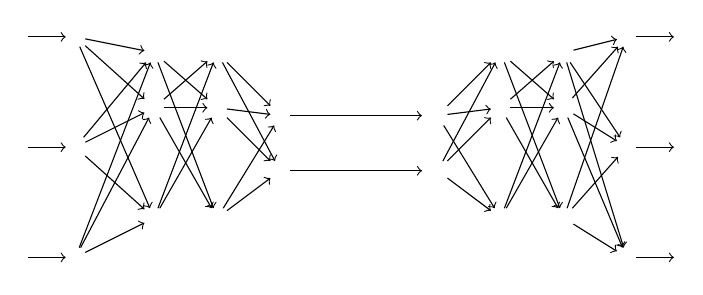
\begin{tikzpicture}
	%encoder
	\foreach \m/\l [count=\y] in {1,missing,3,missing,5}
	\node [neuron/.try, neuron \m/.try] (input1-\m) at (0,2-\y*0.7) {};
	
	\foreach \m [count=\y] in {1,2,missing,4}
	\node [neuron/.try, neuron \m/.try ] (hidden1-\m) at (1,1.8-\y*0.7) {};
	
	\foreach \m [count=\y] in {1,2,missing,4}
	\node [neuron/.try, neuron \m/.try ] (hidden2-\m) at (1.8,1.8-\y*0.7) {};
	
	\foreach \m [count=\y] in {1,2}
	\node [neuron/.try, neuron \m/.try ] (output1-\m) at (2.6,1-\y*0.7) {};
	
	\foreach \i in {1,3}
	\draw [<-] (input1-\i) -- ++(-0.6,0);
	
	\foreach \l [count=\i] in {1,2}
	\draw [->] (output1-\i) -- ++(1.8,0);
%	node [above, midway] {$y_\i$};
	
	
	\draw [<-] (input1-5) -- ++(-0.6,0);

	%mesh1
	\foreach \i in {1,3,5} 
	\foreach \j in {1,2,4}
	\draw [->] (input1-\i) -- (hidden1-\j);
	
	\foreach \i in {1,2,4}
	\foreach \j in {2}
	\draw [->] (hidden1-\i) -- (hidden2-\j);
	
	\draw [->] (hidden1-2) -- (hidden2-1); 
	\draw [->] (hidden1-4) -- (hidden2-1); 
	
	\draw [->] (hidden1-1) -- (hidden2-4); 
	\draw [->] (hidden1-2) -- (hidden2-4); 
	
	\foreach \i in {1,2,4}
	\foreach \j in {1,2}
	\draw [->] (hidden2-\i) -- (output1-\j);
	
	%decoder
	\foreach \m [count=\y] in {1,2}
	\node [neuron/.try, neuron \m/.try ] (input2-\m) at (4.6,1-\y*0.7) {};
	
	\foreach \m [count=\y] in {1,2,missing,4}
	\node [neuron/.try, neuron \m/.try ] (hidden3-\m) at (5.4,1.8-\y*0.7) {};
	
	\foreach \m [count=\y] in {1,2,missing,4}
	\node [neuron/.try, neuron \m/.try ] (hidden4-\m) at (6.2,1.8-\y*0.7) {};
	
	\foreach \m/\l [count=\y] in {1,missing,3,missing,5}
	\node [neuron/.try, neuron \m/.try] (output2-\m) at (7,2-\y*0.7) {};
	
	%outputs
	\foreach \i in {1,3,5}
	\draw [->] (output2-\i) -- ++(0.6,0);
	
	%mesh2
	\foreach \i in {1,2} 
	\foreach \j in {1,2,4}
	\draw [->] (input2-\i) -- (hidden3-\j);
	
	\foreach \i in {1,2,4}
	\foreach \j in {2}
	\draw [->] (hidden3-\i) -- (hidden4-\j);
	
	\draw [->] (hidden3-2) -- (hidden4-1); 
	\draw [->] (hidden3-4) -- (hidden4-1); 
	
	\draw [->] (hidden3-1) -- (hidden4-4); 
	\draw [->] (hidden3-2) -- (hidden4-4); 
	
	\foreach \i in {1,2,4}
	\foreach \j in {1,3,5}
	\draw [->] (hidden4-\i) -- (output2-\j);
	
	
	
	
\end{tikzpicture}    
\end{figure}

You can also use Tikz to display nice plots. You can convert your plot from Python Pyplot to tikz with the command 'import tikzplotlib'
and 'tikzplotlib.save("test.tex")'.
\begin{figure}
    \centering
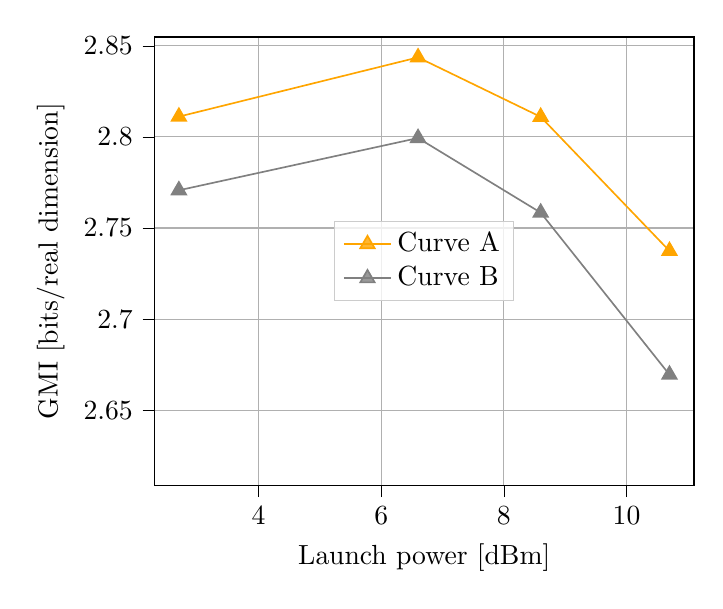
\begin{tikzpicture}

\definecolor{color0}{rgb}{1,0.647058823529412,0}
\definecolor{color1}{rgb}{0.235294117647059,0.701960784313725,0.443137254901961}
\definecolor{color2}{rgb}{0.254901960784314,0.411764705882353,0.882352941176471}

\begin{axis}[
legend cell align={left},
legend style={
  fill opacity=0.8,
  draw opacity=1,
  text opacity=1,
  at={(0.5,0.5)},
  anchor=center,
  draw=white!80!black
},
tick align=outside,
tick pos=left,
x grid style={white!69.0196078431373!black},
xlabel={Launch power [dBm]},
xmajorgrids,
xmin=2.3, xmax=11.1,
xtick style={color=black},
y grid style={white!69.0196078431373!black},
ylabel={GMI [bits/real dimension]},
ymajorgrids,
ymin=2.6087880805, ymax=2.8548327695,
ytick style={color=black}
]
\addplot [semithick, color0, mark=triangle*, mark size=3, mark options={solid}]
table {%
2.7 2.81112629202
6.6 2.84364892
8.6 2.8110044
10.7 2.73741857
};
\addlegendentry{Curve A}
\addplot [semithick, white!50.1960784313725!black, mark=triangle*, mark size=3, mark options={solid}]
table {%
2.7 2.77071057
6.6 2.79938574
8.6 2.75843503
10.7 2.66952503
};
\addlegendentry{Curve B}
\end{axis}

\end{tikzpicture}
\end{figure}

\begin{figure}
% This file was created with tikzplotlib v0.10.1.
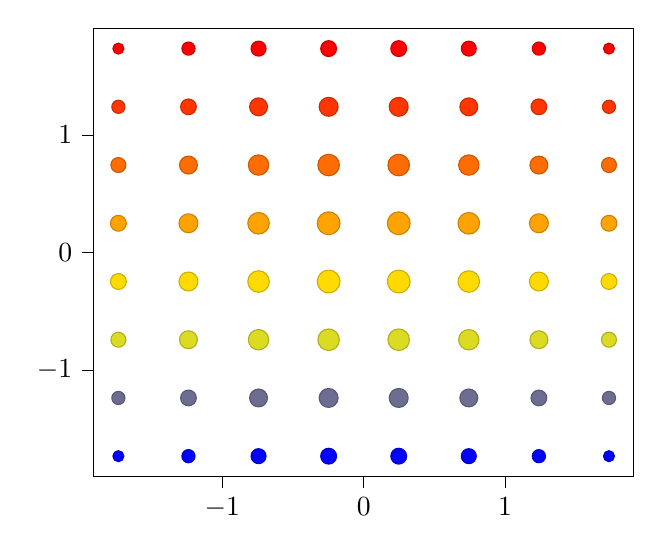
\begin{tikzpicture}

\definecolor{darkgray176}{RGB}{176,176,176}
\definecolor{steelblue31119180}{RGB}{31,119,180}

\begin{axis}[
tick align=outside,
tick pos=left,
x grid style={darkgray176},
xmin=-1.90730187892914, xmax=1.90730187892914,
xtick style={color=black},
y grid style={darkgray176},
ymin=-1.90730187892914, ymax=1.90730187892914,
ytick style={color=black}
]
\addplot [
  draw=steelblue31119180,
  fill=steelblue31119180,
  mark=*,
  only marks,
  scatter,
  scatter/@pre marker code/.append style={/tikz/mark size=\perpointmarksize},
  visualization depends on={\thisrow{sizedata} \as\perpointmarksize}
]
table{%
x  y  sizedata
-1.73391079902649 1.73391079902649 1.9902518
-1.23850774765015 1.73391079902649 2.3760042
-0.743104636669159 1.73391079902649 2.7039983
-0.247701555490494 1.73391079902649 2.8618598
0.247701555490494 1.73391079902649 2.8618598
0.743104636669159 1.73391079902649 2.7039983
1.23850774765015 1.73391079902649 2.3760042
1.73391079902649 1.73391079902649 1.9902518
-1.73391079902649 1.23850774765015 2.3760042
-1.23850774765015 1.23850774765015 2.8365235
-0.743104636669159 1.23850774765015 3.2280898
-0.247701555490494 1.23850774765015 3.416548
0.247701555490494 1.23850774765015 3.416548
0.743104636669159 1.23850774765015 3.2280898
1.23850774765015 1.23850774765015 2.8365235
1.73391079902649 1.23850774765015 2.3760042
-1.73391079902649 0.743104636669159 2.7039983
-1.23850774765015 0.743104636669159 3.2280898
-0.743104636669159 0.743104636669159 3.6737092
-0.247701555490494 0.743104636669159 3.8881829
0.247701555490494 0.743104636669159 3.8881829
0.743104636669159 0.743104636669159 3.6737092
1.23850774765015 0.743104636669159 3.2280898
1.73391079902649 0.743104636669159 2.7039983
-1.73391079902649 0.247701555490494 2.8618598
-1.23850774765015 0.247701555490494 3.416548
-0.743104636669159 0.247701555490494 3.8881829
-0.247701555490494 0.247701555490494 4.115178
0.247701555490494 0.247701555490494 4.115178
0.743104636669159 0.247701555490494 3.8881829
1.23850774765015 0.247701555490494 3.416548
1.73391079902649 0.247701555490494 2.8618598
-1.73391079902649 -0.247701555490494 2.8618598
-1.23850774765015 -0.247701555490494 3.416548
-0.743104636669159 -0.247701555490494 3.8881829
-0.247701555490494 -0.247701555490494 4.115178
0.247701555490494 -0.247701555490494 4.115178
0.743104636669159 -0.247701555490494 3.8881829
1.23850774765015 -0.247701555490494 3.416548
1.73391079902649 -0.247701555490494 2.8618598
-1.73391079902649 -0.743104636669159 2.7039983
-1.23850774765015 -0.743104636669159 3.2280898
-0.743104636669159 -0.743104636669159 3.6737092
-0.247701555490494 -0.743104636669159 3.8881829
0.247701555490494 -0.743104636669159 3.8881829
0.743104636669159 -0.743104636669159 3.6737092
1.23850774765015 -0.743104636669159 3.2280898
1.73391079902649 -0.743104636669159 2.7039983
-1.73391079902649 -1.23850774765015 2.3760042
-1.23850774765015 -1.23850774765015 2.8365235
-0.743104636669159 -1.23850774765015 3.2280898
-0.247701555490494 -1.23850774765015 3.416548
0.247701555490494 -1.23850774765015 3.416548
0.743104636669159 -1.23850774765015 3.2280898
1.23850774765015 -1.23850774765015 2.8365235
1.73391079902649 -1.23850774765015 2.3760042
-1.73391079902649 -1.73391079902649 1.9902518
-1.23850774765015 -1.73391079902649 2.3760042
-0.743104636669159 -1.73391079902649 2.7039983
-0.247701555490494 -1.73391079902649 2.8618598
0.247701555490494 -1.73391079902649 2.8618598
0.743104636669159 -1.73391079902649 2.7039983
1.23850774765015 -1.73391079902649 2.3760042
1.73391079902649 -1.73391079902649 1.9902518
};
\end{axis}

\end{tikzpicture}

\end{figure}

\end{document}
